\documentclass{article}

\usepackage{fullpage}
\usepackage{color}
\usepackage{amsmath}
\usepackage{url}
\usepackage{verbatim}
\usepackage{graphicx}
\usepackage{parskip}
\usepackage{amssymb}
\usepackage{nicefrac}
\usepackage{listings} % For displaying code
\usepackage{algorithm2e} % pseudo-code

% Answers
\def\ans#1{\par\gre{Answer: #1}}
%\def\ans#1{} % Comment this line to produce document with answers

% Colors
\definecolor{blu}{rgb}{0,0,1}
\def\blu#1{{\color{blu}#1}}
\definecolor{gre}{rgb}{0,.5,0}
\def\gre#1{{\color{gre}#1}}
\definecolor{red}{rgb}{1,0,0}
\def\red#1{{\color{red}#1}}
\def\norm#1{\|#1\|}

% Math
\def\R{\mathbb{R}}
\def\argmax{\mathop{\rm arg\,max}}
\def\argmin{\mathop{\rm arg\,min}}
\newcommand{\mat}[1]{\begin{bmatrix}#1\end{bmatrix}}
\newcommand{\alignStar}[1]{\begin{align*}#1\end{align*}}
\def\half{\frac 1 2}
\def\cond{\; | \;}

% LaTeX
\newcommand{\fig}[2]{\includegraphics[width=#1\textwidth]{a6f/#2}}
\newcommand{\centerfig}[2]{\begin{center}\includegraphics[width=#1\textwidth]{a6f/#2}\end{center}}
\def\items#1{\begin{itemize}#1\end{itemize}}
\def\enum#1{\begin{enumerate}#1\end{enumerate}}


\begin{document}

\title{CPSC 340 Assignment 6 (due Friday November 29 at 11:55pm)}
\author{Zijia Zhang 42252965}
\date{}
\maketitle
\vspace{-2em}


\section{Robust PCA}


The function \emph{example\_RPCA} loads a dataset $X$ where each row contains the pixels from a single frame of a video of a highway. The demo applies PCA to this dataset and then uses this to reconstruct the original image. It then shows the following 3 images for each frame of the first 50 frames (pausing for a tenth of a second on each frame):
\enum{
\item The original frame.
\item The reconstruction based on PCA.
\item A binary image showing locations where the reconstruction error is non-trivial.
}
Recently, latent-factor models have been proposed as a strategy for ``background subtraction'': trying to separate objects from their background. In this case, the background is the highway and the objects are the cars on the highway. In this demo, we see that PCA does an ok job of identifying the cars on the highway in that it does tend to identify the locations of cars. However, the results aren't great as it identifies quite a few irrelevant parts of the image as objects.

Robust PCA is a variation on PCA where we replace the L2-norm with the L1-norm,
\[
f(Z,W) = \sum_{i=1}^n\sum_{j=1}^d |w_j^Tz_i - x_{ij}|,
\]
and it has recently been proposed as a more effective model for background subtraction. \blu{Write a new function, \emph{robustPCA}, that uses the Huber loss to approximate the absolute value to implement robust PCA. Hand in your code.}

Hint: most of the work has been done for you in the function \emph{PCA\_gradient}. This function  implements an alternating minimization approach to minimizing the PCA objective (without enforcing orthogonality). This gradient-based approach to PCA can be modified to use the Huber loss. A reasonable value of the hyper-parameter $\epsilon$ in the Huber loss might be $0.01$ for this problem. You may want to use a smaller version of the dataset when debugging your objective/gradient code.
\ans{\\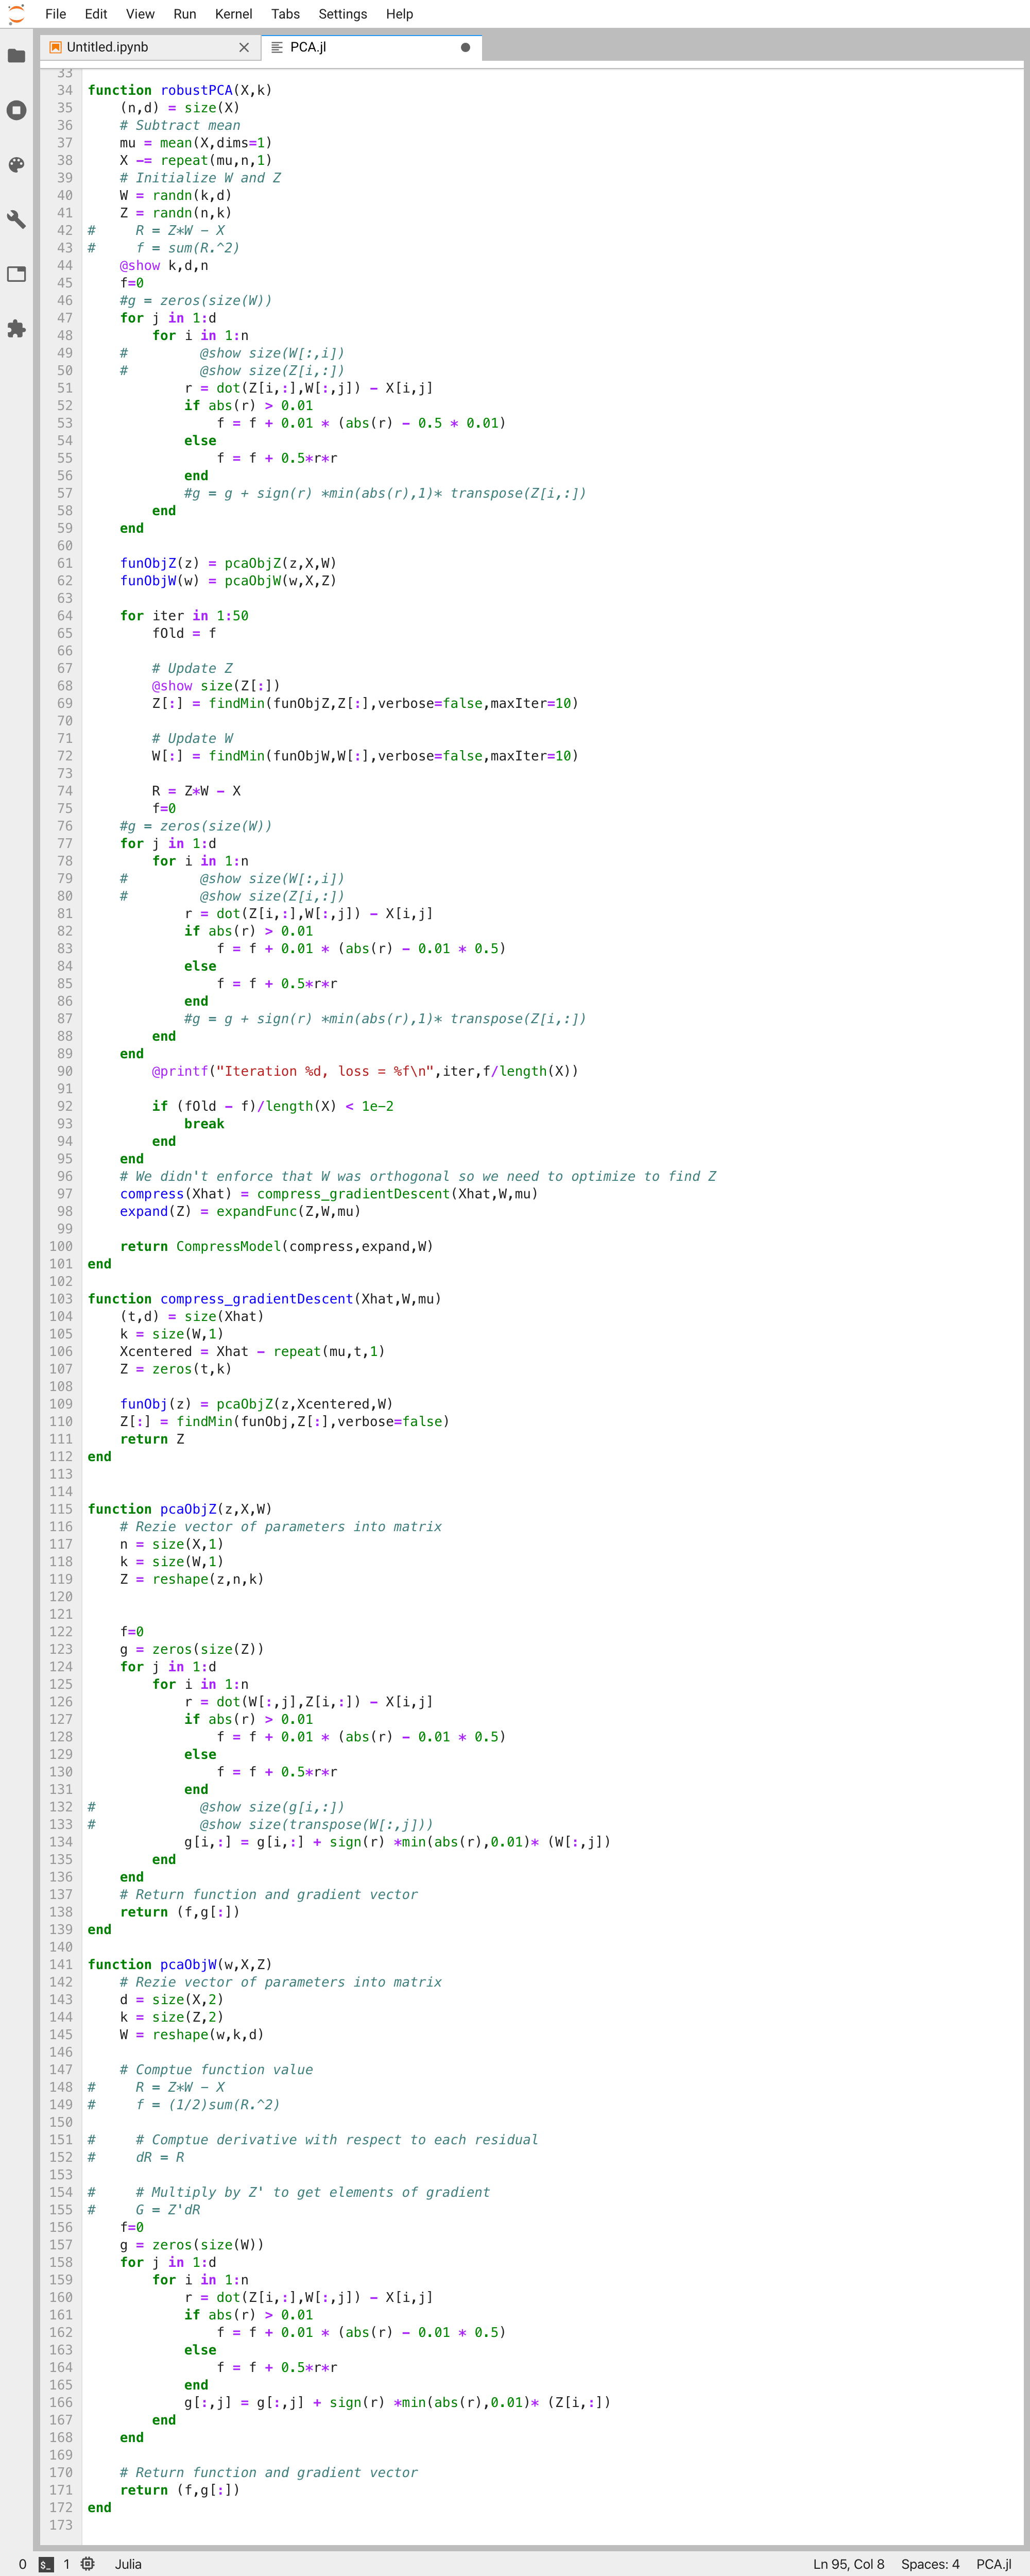
\includegraphics[width=10cm]{Q11Code2.png} \\ 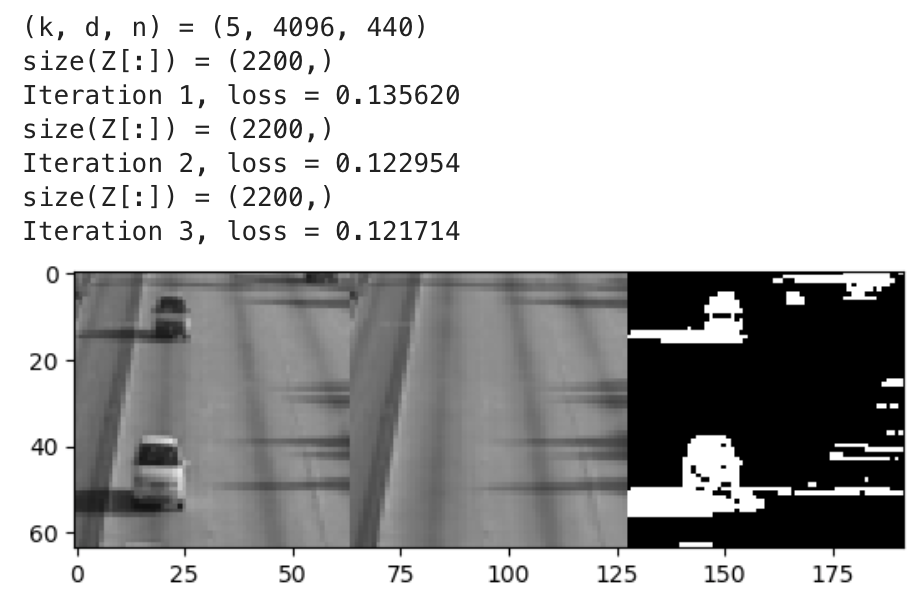
\includegraphics[width=10cm]{Q11Result.png}}



\section{Multi-Dimensional Scaling}

The function \emph{example\_MDS} loads the animals dataset and then applies gradient dsecent to minimize the following multi-dimensional scaling (MDS) objective (starting from the PCA solution):
\begin{equation}
\label{eq:MDS}
f(Z) =  \frac{1}{2}\sum_{i=1}^n\sum_{j=i+1}^n (  \norm{z_i - z_j} - \norm{x_i - x_j})^2.
\end{equation}
 The result of applying MDS is shown below.
Although this visualization isn't perfect (with ``gorilla'' being placed close to the dogs and ``otter'' being placed close to two types of bears), this visualization does organize the animals in a mostly-logical way.


\subsection{ISOMAP}

Euclidean distances between very different animals are unlikely to be particularly meaningful. However, since related animals tend to share similar traits we might expect the animals to live on a low-dimensional manifold. This suggests that ISOMAP may give a better visualization. Make a new function \emph{ISOMAP} that computes the approximate geodesic distance (shortest path through a graph where the edges are only between nodes that are $k$-nearest neighbour) between each pair of points, and then fits a standard MDS model~\eqref{eq:MDS} using gradient descent. \blu{Hand in your code and the plot of the result when using the $3$-nearest neighbours}.
\ans{\\
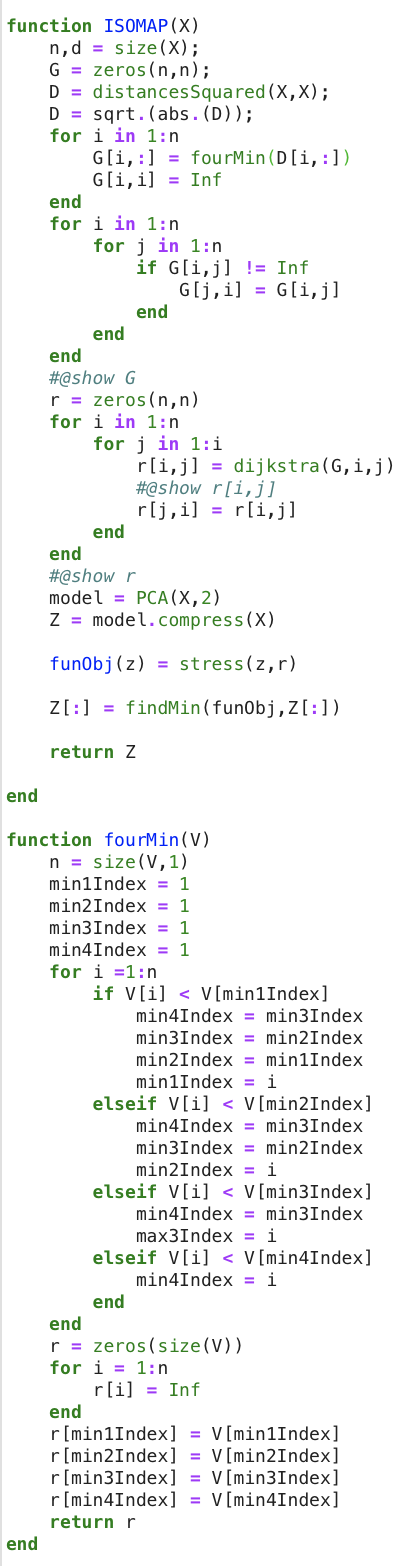
\includegraphics[width=5cm]{Q21.png} \\
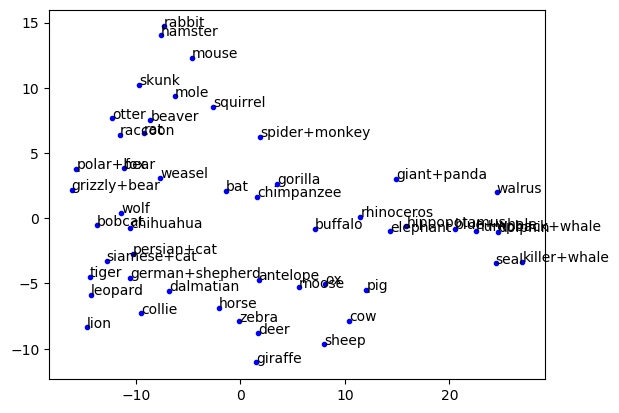
\includegraphics[width=10cm]{Q21img.png}} \\
Hint: the function \emph{dijskstra} (in \emph{misc.jl}) can be used to compute the shortest (weighted) distance between two points in a weighted graph. This function requires an $n$ by $n$ matrix giving the weights on each edge (use $\infty$ as the weight for absent edges). Note that ISOMAP uses an undirected graph, while the $k$-nearest neighbour graph might be asymmetric. You can use the usual heuristics to turn this into an undirected graph of including an edge $i$ to $j$ if $i$ is a KNN of $j$ or if $j$ is a KNN of $i$. (Also, be careful not to include the point itself in the KNN list).




\subsection{ISOMAP with Disconnected Graph}

An issue with measuring distances on graphs is that the graph may not be connected. For example, if you run your ISOMAP code with $2$-nearest neighbours then some of the distances are infinite. One heuristic to address this is to set these infinite distances to the maximum distance in the graph (i.e., the maximum geodesic distance between any two points that are connected), which will encourage non-connected points to be far apart. Modify your ISOMAP function to implement this heuristic. \blu{Hand in your code and the plot of the result when using the $2$-nearest neighbours}.
\ans{
    \\
    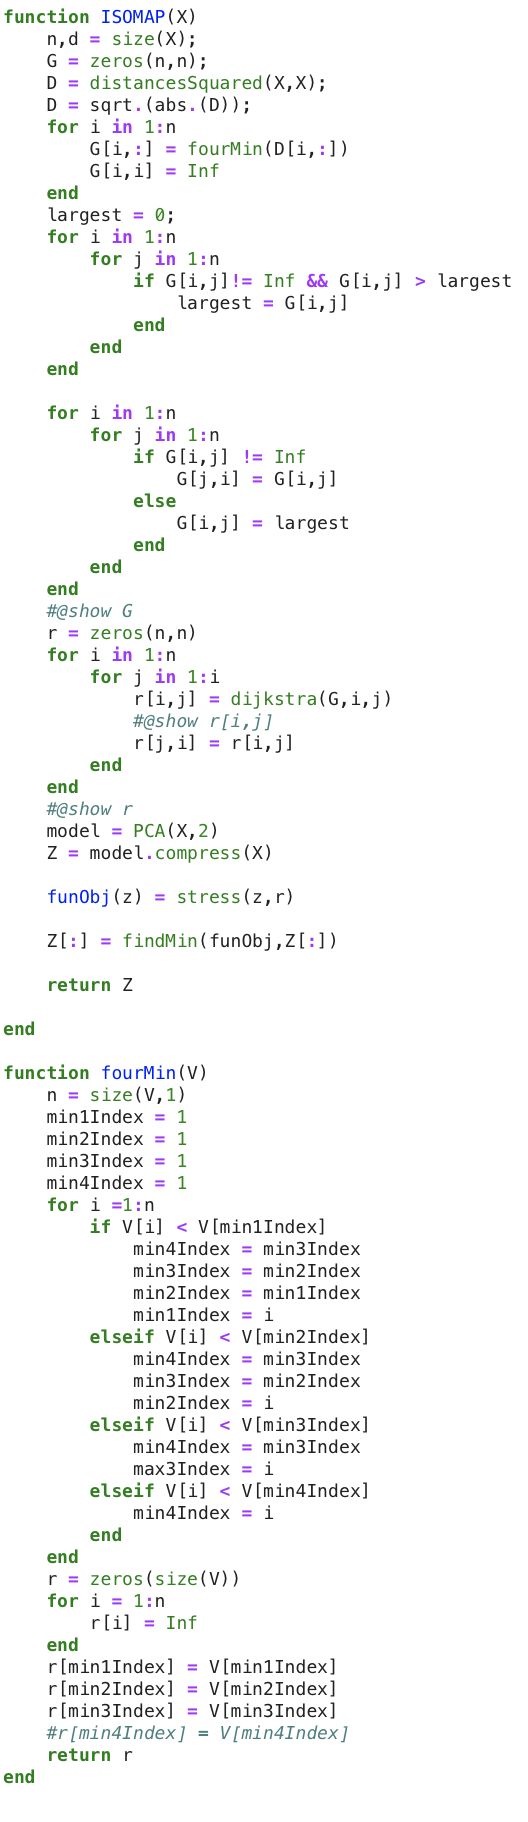
\includegraphics[width = 5cm]{Q22Code.png}
    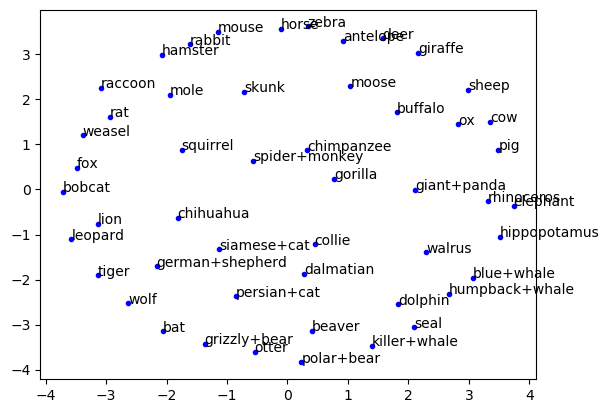
\includegraphics[width = 10cm]{Q22Graph.png}}



\section{Neural Networks}


\subsection{Neural Networks by Hand}

Suppose that we train a neural network with sigmoid activations and one hidden layer and obtain the following parameters (assume that we don't use any bias variables):
\[
W = \mat{-2 & 2 & -1\\1 & -2 & 0}, v = \mat{3 \\1}.
\]
Assuming that we are doing regression, \blu{for a training example with features $x_i^T = \mat{-3 &-2 & 2}$ what are the values in this network of $z_i$, $h(z_i)$, and $\hat{y}_i$?}
\ans{
    $z_i = Wx_i = [0, 1]$ \\
    $h(z_i) = [0.5, e/(e+1)]$ \\
    $y = 1.5 + e/(e+1)$
}
\subsection{Neural Network Tuning - Regression}

The file \texttt{example\_nnet.jl} runs a stochastic gradient method to train a neural network on the \emph{basisData} dataset from a previous assignment. However, in its current form it doesn't fit the data very well. Modify the training procedure to improve the performance of the neural network. \blu{Hand in your plot after changing the code to have better performance, and list the changes you made}.
\ans{
    Change the number of layers to 10000. Change to 15000 steps and stepsize to 1e-5.
    \\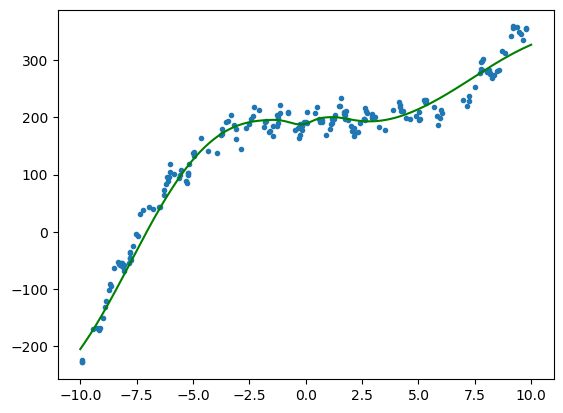
\includegraphics[width=10cm]{Q32.png}
    }

Hint: there are many possible strategies you could take to improve performance. Below are some suggestions, but note that the some will be more effective than others:
\items{
\item Changing the network structure (\emph{nHidden} is a vector giving the number of hidden units in each layer).
\item Changing the training procedure (you can change the stochastic gradient step-size, use mini-batches, run it for more iterations, add momentum, switch to \emph{findMin}, and so on).
\item Transform the data by standardizing the feautres, standardizing the targets, and so on.
\item Add regularization (L2-regularization, L1-regularization, dropout, and so on).
\item Add bias variables within the hidden layers.
\item Change the loss function or the non-linearities (right now it uses squared error and $\tanh$ to introduce non-linearity).
\item Use mini-batches of data, possibly with batch normalization.
}

\subsection{Neural Network Tuning - Classification}

The file \texttt{example\_usps.jl} runs a stochastic gradient method to train a neural network on a set of images of digits. Modify the training procedure to improve the performance of the neural network. \blu{List the changes you made and the best test performance that you were able to obtain}.
\ans{Tried 2 ways to improve the performance: 
\\1. Change the number of hidden unit to 1000. Achived a testing error of 0.131 with maxIter = 48000.
\\2. Perform PCA first with k = 100 and change the number of unit in the layer to 200. Changed step size to 1e-4 when reaches 30000 iterations and 1e-5 when reaches 50000 iterations. At max iterations of 150000, achived test error of 0.128.}

\section{Very-Short Answer Questions}


\blu{
\enum{
\item Is the NMF loss function convex? What is an optimization method you could use to try to minimize it? \ans{No, we can use Projected-Gradient to solve this kind of problem.}
\item Consider fitting a linear latent-factor model, using L1-regularization of the $w_c$ values and L2-regularization of the $z_i$ values,
\[
f(Z,W) = \frac{1}{2}\norm{ZW - X}_F^2 + \lambda_W \sum_{c=1}^k \left[\norm{w_c}_1\right] + \frac{\lambda_Z}{2} \sum_{i=1}^n \left[\norm{z_i}^2\right],
\]
\enum{
\item What is the effect of $\lambda_Z$ on the two parts of the fundamental trade-off in machine learning? \ans{When $\lambda _Z$ is big, the training error will increase and approximation error will decrease.}
\item What is the effect of $k$ on the two parts? \ans{When k increases, the training error will decrease, and approximation error will increase.}
\item Would either of answers to the \emph{previous two questions} change if $\lambda_W = 0$? \ans{(1) The $\lambda_Z$ will not affect. (2) k will have the same effect.}
}
\item Which is better for recommending movies to a new user, collaborative filtering or content-based filtering? Briefly justify your answer.
\ans{content-based filtering, because colaborative filtering need to depend on finding similarities in teh ratings, but new users don't have any.}
\item Is ISOMAP mainly used for supervised or unsupervised learning? Is it parametric or non-parametric?
\ans{Unsupervised, is non-parametric model.}
\item What is the difference between Euclidean distance and geodesic distance?
\ans{Geodesic distance requires the distance to go through neighbouring points, whereas the Euclidean distance does not enforce that.}
\item Are neural networks mainly used for supervised or unsupervised learning? Are they parametric or nonparametric?
\ans{Supervised, parametric}
\item The loss for a neural network is typically non-convex. Give one set of hyperparameters for which the loss is actually convex.
\ans{nLayers = [1] h(x) = x}
\item Assuming we have some procedure that returns a random global minimum of a neural network objective, how does the depth of a neural network affect the fundamental trade-off? For a convolutional network, how would the width of the convolutions affect the fundamental trade-off?
\ans{The deeper the Network is, the lower training error it gets, but the approximation error goes higher, For convolutional network, the wider the convolutions are, the bigger training error it gets and the lower the approximation it gets.}
\item What is the ``vanishing gradient'' problem with neural networks based on sigmoid non-linearities?
\ans{When the sigmoid function is far away from 0, the gradiant will be approach 0, which might cause underflow, so the gradiant becomes 0.}
\item List 3 forms of regularization we use to prevent overfitting in neural networks.
\ans{L2 regularization, Early Stopping, SGD}
\item Convolutional networks seem like a pain... why not just use regular (``fully connected'') neural networks for image classification?
\ans{Because it can represents the relationship between features, so they are not independent to each other. So it can reduce the time of training and overfitting.}
}
}




\end{document}